\documentclass[article, backcover, nodocumentinfo, french]{upmethodology-document}

%% The TeX code is entering with UTF8
%% character encoding (Linux and MacOS standards)
\usepackage[utf8]{inputenc}
%% For algorithms
\usepackage[chapter]{algorithm}
\usepackage{algpseudocode}
%% For bibtex
\usepackage{natbib}

%% For trees
\usepackage[linguistics]{forest}

%% For cute boxes
\usepackage{fancybox}

\usepackage{color}

% for index
\usepackage{makeidx}

\setdocabstract{}

\makeatletter
\let\VERversion\upm@package@version@ver
\let\VERfmt\upm@package@fmt@ver
\let\VERdoc\upm@package@doc@ver
\let\VERfp\upm@package@fp@ver
\let\VERbp\upm@package@bp@ver
\let\VERext\upm@package@ext@ver
\let\VERtask\upm@package@task@ver
\let\VERdocclazz\upm@package@docclazz@ver
\let\VERcode\upm@package@code@ver
\makeatother

% Espace insécable (le caractère ~ se traduit par un espace insécable).
\DeclareUnicodeCharacter{00A0}{~}
% Sur un clavier bépo, on a un accès direct au ×
\DeclareUnicodeCharacter{00D7}{\times}

\newcommand{\notion}[1]{{\slshape{}\large{}\color{red}#1}}

\newcommand{\tl}{\textless}
\newcommand{\tg}{\textgreater}

\newcommand{\bb}[1]{\mathbb{#1}} % the blackboard bold capital is used for sets.



\declaredocument{Rapport de projet LO41}{Livraison de colis par drone}{LO41-P2017}

\setfrontcover{classic}

\addauthorvalidator*[benoit.cortier@utbm.fr]{Benoît}{CORTIER}{Author}
\addauthorvalidator*[lucas.lazare@utbm.fr]{Lucas}{LAZARE}{Author}

\setcopyrighter{Benoît CORTIER \& Lucas Lazare}
\setprintingaddress{France}

\setpublisher{University of Technology of Belfort-Montbéliard}

%% jj/mm/yyyy
\incversion{\makedate{09}{06}{2017}}{Initial version.}{\upmpublic}
\incversion{\makedate{09}{06}{2017}}{Last update.}{\upmpublic}

\setdockeywords{LO41, drone, simulation, livraison, \LaTeX}

\makeindex

\graphicspath{{./fig/}}

% to include only those
%\includeonly{./tex/introduction, ./tex/elementary}

\begin{document}

\chapter{Introduction}



\section{Modélisation avec diagramme de Pétri}

\begin{figure}[H]
    \centering
    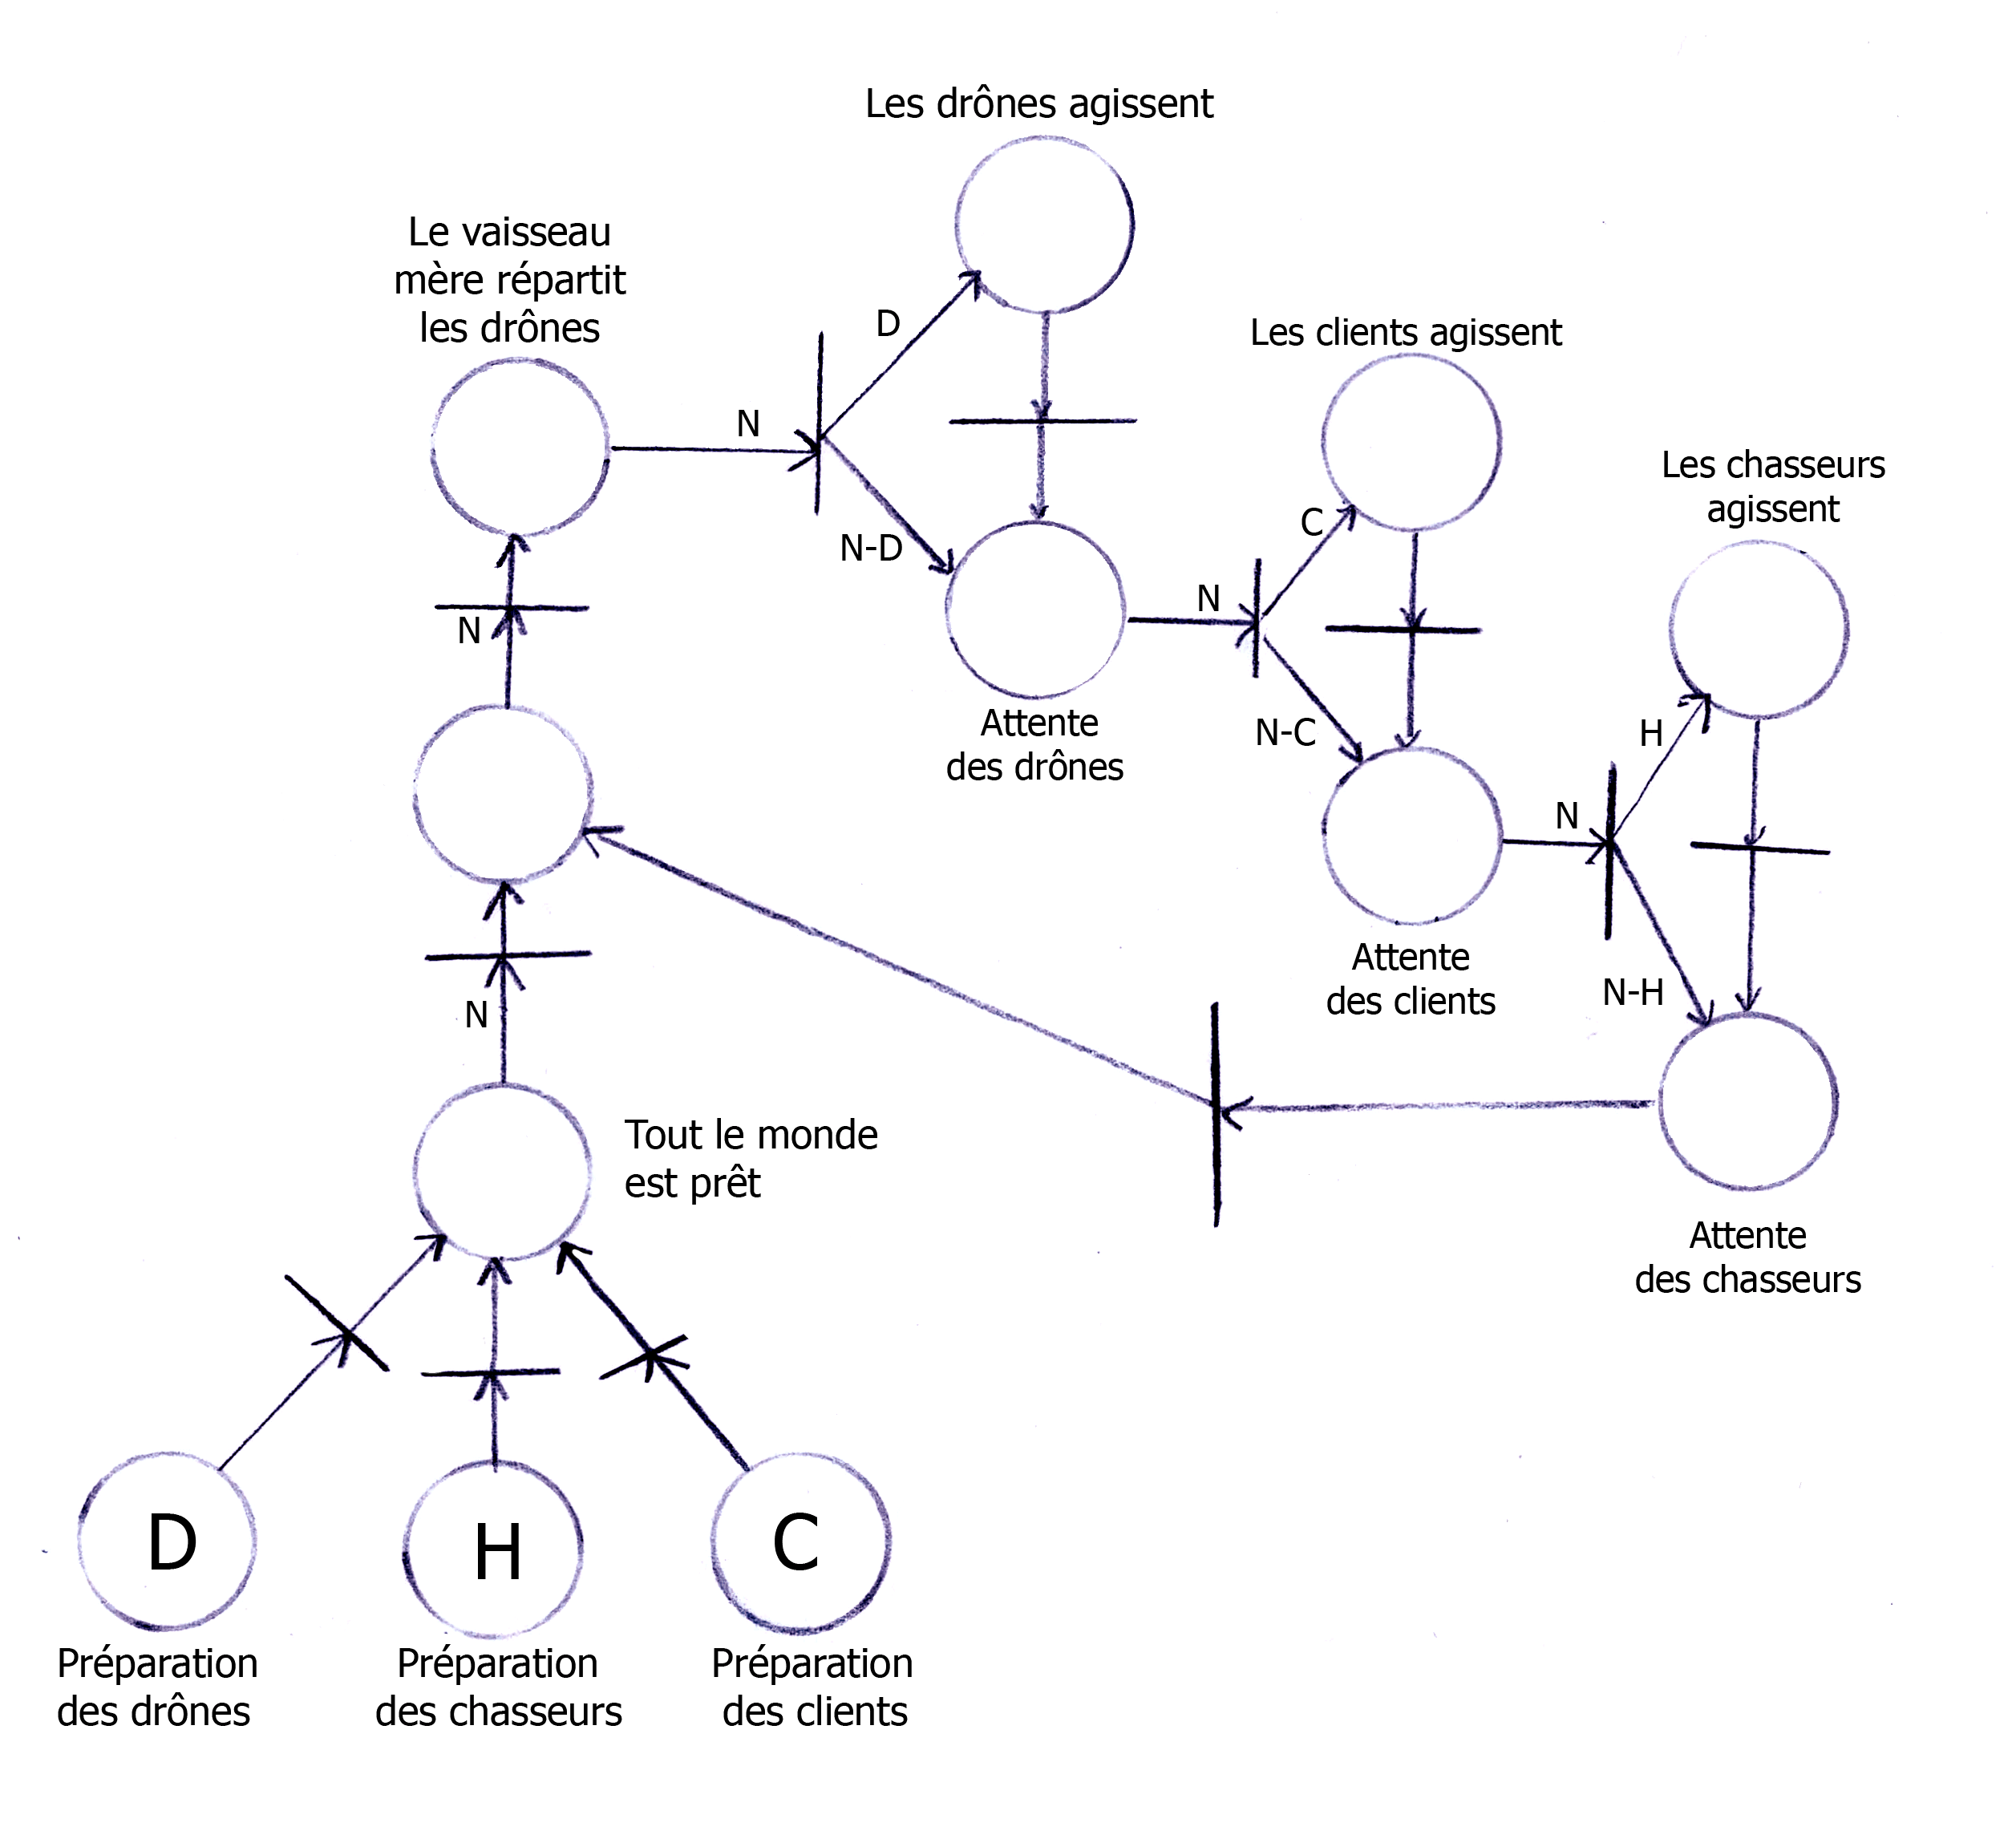
\includegraphics[width=.67\linewidth]{PTREE2}
    \caption{Modélisation du système d'horloge de la simulation : fonctionnement global}
\end{figure}

\begin{figure}[H]
    \centering
    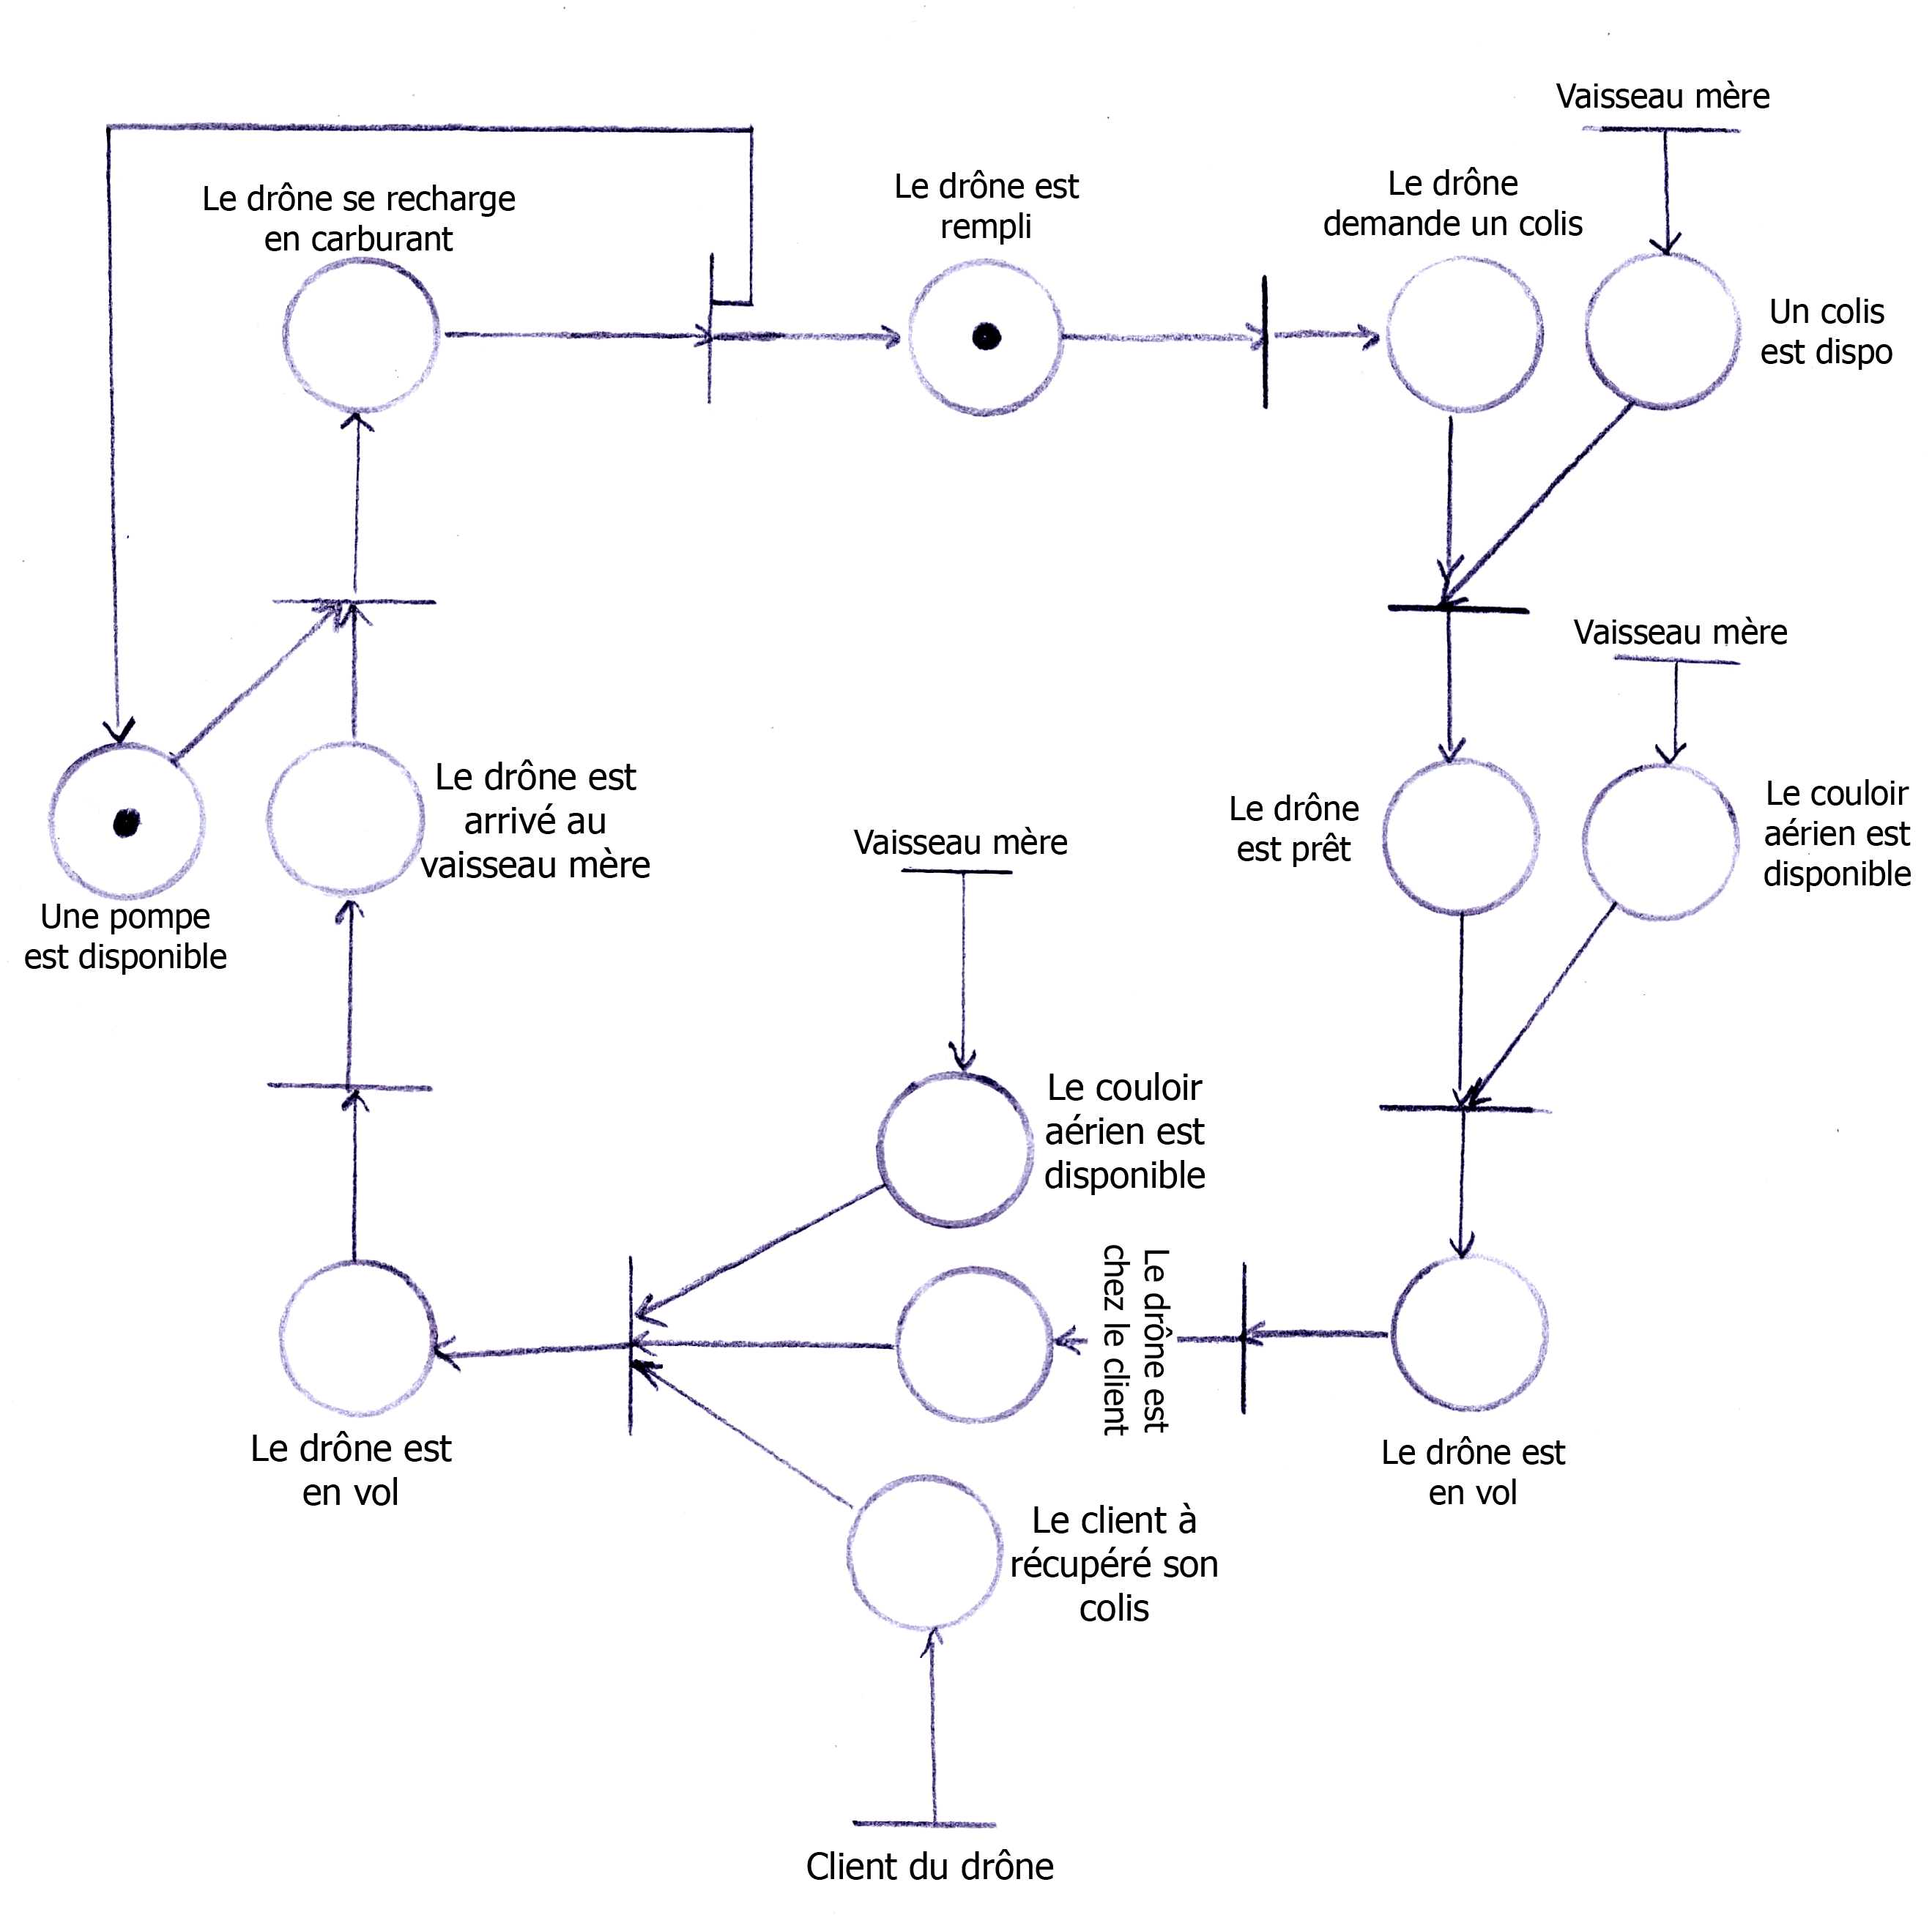
\includegraphics[width=.67\linewidth]{PTREE1}
    \caption{Fonctionnement détaillé du comportement voulu d'un drône}
\end{figure}



\section{Synchronisation et communication}

Tout d'abord, nous avons fait le choix d'utiliser les processus et non les threads.
Le vaisseau mère est le processus père de tous les autres processus : processus drone, processus client et processus chasseur.
De ce fait, tous les éléments sont réellement indépendants les uns des autres et il est nécessaire de communiquer via
des objets IPC : pas de partage de l'espace d'adressage comme pour les threads (qui n'auraient alors nécessité que
la mise en place de verroux pour la synchronisation). Cela nous a semblé plus proche
du comportement final du système de livraison. Il est possible d'envoyer manuellement le signal \codequote{SIGKILL} à un processus
drone et la simulation s'adaptera, de la même façon que dans la réalité un drone peut avoir dysfonctionnement.
Des événements tels que les chasseurs (processus tueurs de drones) sont également présents pour simuler cela.
La gestion des signaux avec les processus est bien plus commode.

Pour la synchronisation de la simulation, nous avons mis en place un système d'horloge et de pas de simulation. Un pas
de simulation correspond à un tic d'horloge. Lors un pas de simulation, les différents processus effectuent des tâches
bien précises et attendent le pas suivant. Ainsi, on est sûrs que tout le monde effectue à temps équivalent la même
quantité d'action. De plus, il est possible de ralentir ou d'accelerer la simulation selon la vitesse de l'horloge.

Nous utilisons la plupart des objets IPC : \emph{signaux, tubes, sémaphores, mémoire partagée et file de messages.}

Les \emph{signaux} sont utilisés dans diverses portions du programme :
\begin{itemize}
    \item gestion de l'interruption clavier.
    \item meurtre de drone (par les chasseurs) avec \codequote{SIGKILL}.
    \item écoute des processus enfants qui s'arrêtent par le vaisseau mère (cf: chapitre \ref{chap:mothership}).
    \item indication à un processus précis de se remettre à travailler (exécution d'un tic d'horloge) avec un signal utilisateur
        envoyé par le vaisseau mère (cf: chapitre \ref{chap:mothership}).
\end{itemize}

Nous utilisons une seule \emph{sémaphore} pour permettre au vaisseau mère d'attendre les processus qui travaillent. Lorsqu'un
processus a terminé son tic d'horloge, il incrémente la valeur de la sémaphore.

Les \emph{tubes} sont utilisés pour la communication drones/clients.
Les clients ouvrent tous une paire de tubes (un pour la lecture, l'autre pour l'écriture).
Lorsqu'un drone veut communiquer avec un client, il écrit simplement dans le bon tube et attend la réponse dans l'autre tube.

Le \emph{segment de mémoire partagée} est utilisé pour compter et stocker une liste de drones actuellement dans les airs.
Le vaisseau mère tient cette liste à jour et les chasseurs piochent dans la liste pour tuer des drones aléatoirement.

La \emph{file de messages} est utilisée pour la communication vaisseau mère/drones. Le type des messages correspond au pid des
destinataire. Ainsi, chacun peut récupérer les messages qui lui sont destinés et travailler selon.



\chapter{Fonctionement du vaisseau mère}\label{chap:mothership}

Le processus du vaisseau mère est le parent de tous les autres processus de type drone, client ou chasseur.
Il connaît le pid de tout le monde et est en mesure de surveiller l'état de tout le monde. Il écoute le signal SIGCHLD pour
être notifié si un processus meurt et de quelle façon : selon ce qui se produit, il s'assure que la simulation peut
continuer sans problème en mettant à jour certaines données ou bien stoppe la simulation et nettoie la mémoire.
Il s'occupe aussi de gérer l'interruption (ctrl+C) : nettoyage de la mémoire et envoi d'un signal d'extinction aux enfants.

C'est aussi lui qui gère la synchronisation et le pas de simulation :
nous utilisons une sémaphore POSIX pour faire dormir le vaisseau mère et attendre qu'un certain nombre de processus aient
terminé leur pas de simulation. Puis, le vaisseau mère lit les messages qui lui sont destinés et effectue les
tâches associées. Une fois la lecture des messages terminée, le vaisseau mère envoie un signal
aux processus qui peuvent se remettre à travailler.

Le vaisseau mère fait travailler les processus dans un ordre bien précis : c'est d'abord les processus drones qui
se remettent à travailler, puis les processus clients et enfin les processus chasseurs.
L'ordre a une certaine importance dans la mesure où :
\begin{itemize}
    \item les chasseurs ne peuvent tirer sur un drone que si celui-ci est dans les airs.
    \item si un drone veut communiquer avec le client, la lecture étant non bloquante (pour les besoins de l'horloge de simulation),
        le plus efficace est de faire en sorte d'envoyer le message en premier. Ainsi, l'envoie et la lecture du message a lieu
        au même tic d'horloge. Ceci a du sens dans la mesure où ce n'est jamais le client qui initie la communication avec le
        drone, mais toujours le drone qui initie la communication avec le client.
\end{itemize}

Le vaisseau mère et les drones communiquent également via une file de messages System V qui,
contrairement à la file de messages POSIX, permet de donner un type aux messages. Nous utilisons
le type pour indiquer le pid du destinataire du message.

Au niveau de la simulation en elle même, le vaisseau mère s'occupe d'un certain nombre de tâches importantes :
\begin{itemize}
    \item autoriser le \emph{décollage et le départ des drones}. Pour pouvoir partir, un drone doit nécessairement envoyer
        une requête au vaisseau mère qui pourra ou non l'autoriser à partir selon la disponibilité des couloirs aériens.
    \item fournir des emplacements de \emph{recharche de batterie} aux drones qui le demandent.
    \item fournir un \emph{colis approprié} aux drones. Lorsqu'un drone demande un colis, le vaisseau mère sélectionne un colis
        selon plusieurs critères : le contenance et le poids maximal que le drone peut porter ainsi que son autonomie.
        De plus, sur plusieurs colis appropriés, c'est celui dont la priorité est la plus élevée qui est sélectionné.
    \item \emph{garder une trace des différents évènements} qui se produisent :
        colis livrés, à livrer et perdus, couloirs aériens utilisés, drones disponibles, en vol, perdus, …
\end{itemize}

La liste des drones en vol est dans un segment de mémoire partagée (objet POSIX) et c'est le vaisseau mère
qui s'assure de la tenir à jour. Aucun verrou n'est nécessaire sur les modifications de cette liste car le vaisseau mère
ne la modifie que lorsque tous les autres processus sont endormis en attente du signal de reprise. La synchronisation est donc
déjà gérée.



\section{Fonctionement des drones}

Chaque drone est un processus à part entière, de la même manière que le vaisseau mère, les clients, et les chasseurs.
Tout les drônes attendent l'arrivée du tic du vaisseau mère, et agissent alors parallèlement, selon leur état courant.
Les drone sont en effet des \emph{Automates fini}, mis en place à l'aide de pointeurs vers des fonctions.

Les différents états sont les suivants:
\begin{itemize}
    \item en vol
    \item livraison du colis
    \item rechargement en carburant
    \item chargement du colis
    \item attente d'autorisation de départ.
\end{itemize}

\subsection{État `En vol'}
    Lorsqu'un drone est en vol, il consomme une unité de carburant par tic, et avance de sa N unités de distance vers sa cible,
    le client ou le vaisseau mère (avec N la vitesse du drone).
    Si sa réserve de caburant arrive à \(0\), le drone se crashe alors via un \codequote{exit(CRASHED)},
    et le vaisseau mère peut alors récupérer l'information avec un \codequote{wait}. \\
    Une fois que le vol est terminé, le drone signale au vaisseau mère son arrivée via une file de messages,
    et passe dans l'état `livraison du colis' si le drone est parvenu au client qu'il doit livrer,
    ou `rechargement en carburant' s'il vient d'arriver au vaisseau mère.

\subsection{État `Livraison du colis'}
    Dans l'état `livraison du colis', le drone se pose chez son client et l'informe de son arrive.
    Après cela, il reste en attente jusqu'à ce que son client cible ait finit de récupérer son colis.
    Une fois son client livré, il passe à l'état `Attente d'autorisation de départ', afin de ne pas
    percuter un autre drone qui utiliserai le même couloir aérien.

\subsection{État `Attente d'autorisation de départ'}
    Avant de décoller du vaisseau mère ou de revenir de chez le client, le drone demande au vaisseau mère
    l'autorisation de décoller, pour empêcher deux accidents possible:
    \begin{itemize}
        \item collision entre deux appareils utilisant le même couloir aérien
        \item un client n'a pas fini de récupérer son colis (on ne sait pas combien de temps il va encore prendre).
    \end{itemize}
    Un fois qu'il a obtenu l'autorisation de partir, le drone s'en va vers sa destination, et passe dans l'état `en vol'.

\subsection{État `Rechargement en carburant'}
    Pour se recharger en carburant, le drone demande tout d'abord au vaisseau mère un câble de recharge.
    S'il n'y en a pas de disponible, le drone redemande alors câble au tic suivant.
    Une fois de câble obtenu, le drone attend d'être completement chargé, libère le câble,
    et passe dans l'état `chargement du colis'.

\subsection{État `Chargement du colis'}
    Dans cet état, le drône demande au vaisseau mère de lui fournir un colis.
    Il y a alors trois possibilités:
    \begin{itemize}
        \item aucun bras de chargement n'est dispnible, auquel cas le drone attend le tic suivant
        \item aucun colis adapté au drone n'est disponible, auquel cas le drone est éteind.
        \item un colis est disponible, et est alors chargé sur le drone.
    \end{itemize}
    Si le drone a acqui un colis, il passe alors dans l'état `Attente d'autorisation de départ',
    avant de s'élancer vers son client cible.



\end{document}

